\subsubsection{ESP32 Devkit-C}

 El ESP32 Devkit-C es una placa de desarrollo compacta y versátil basada en el microcontrolador ESP32 de Espressif Systems, una solución popular en el ámbito de los sistemas embebidos y aplicaciones IoT \cite{esp32}. Este módulo está diseñado para ofrecer una plataforma accesible para el desarrollo de aplicaciones que requieren conectividad Wi-Fi \cite{ieee_802.11} y Bluetooth \cite{bluetooth}, así como capacidades de procesamiento avanzadas. En la figura \ref{fig:esp32}
 se puede visualizar el módulo ESP32 Devkit-C. \\

 
\begin{figure}[H]
    \centering
    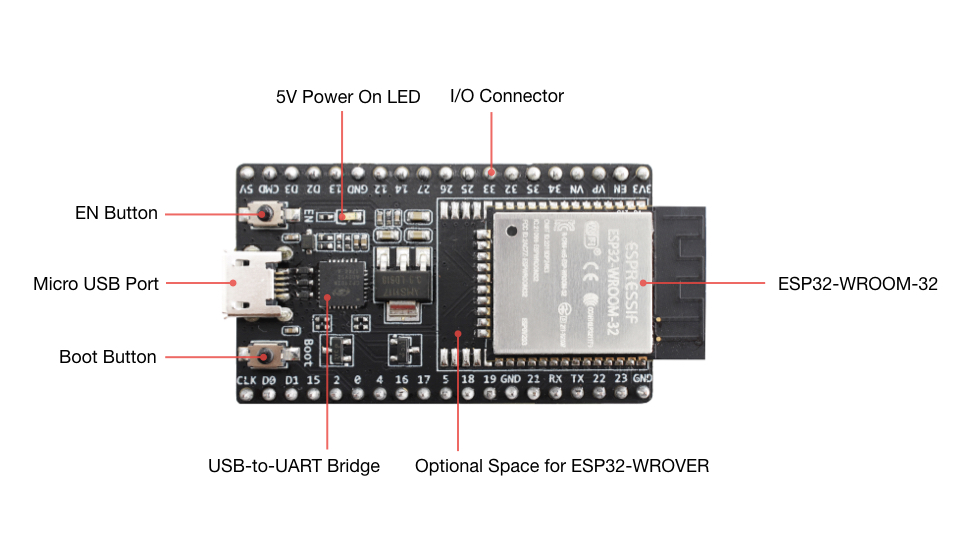
\includegraphics[width=\linewidth]{img/esp32.jpg}
    \caption{Placa de desarrollo ESP32 Devkit-C}
    \label{fig:esp32}
\end{figure}

 
Algunas de las características principales del ESP32 son las siguientes:
\begin{itemize}
    \item \textbf{Microcontrolador dual-core}: cuenta con un procesador dual-core Xtensa LX6 que opera a una velocidad de hasta 240 MHz. Esta arquitectura multiprocesador permite ejecutar tareas paralelas, lo que resulta ventajoso en aplicaciones donde es necesario manejar múltiples procesos simultáneamente, como la gestión de comunicaciones y control de dispositivos.
    \item \textbf{Conectividad inalámbrica}: uno de los aspectos más destacados del ESP32 es su capacidad de conectividad inalámbrica:
        \begin{itemize}
            \item \textbf{Wi-Fi 802.11 b/g/n}: incluye un módulo Wi-FI integrado que permite conectarse a redes inalámbricas, ya sea como cliente o como punto de acceso.
            \item \textbf{Bluetooth 4.2 (BLE y clásico)}: soporta Bluetooth de baja energía (BLE) y Bluetooth clásico, lo que facilita la comunicación con una amplia variedad de dispositivos, desde teléfonos móviles hasta sensores y actuadores.
        \end{itemize}
    \item \textbf{Amplia gama de interfaces de comunicación}: ofrece varias interfaces periféricas, lo que lo hace adecuado para interactuar con otros dispositivos y sensores (UART, SPI, I2C, CAN, PWM, ADC y DAC).
    \item \textbf{Memoria}: incluye 520 KB de SRAM y hasta 16 MB de flash externa, lo que le permite ejecutar aplicaciones complejas y almacenar datos de manera eficiente. Esta combinación de memoria es adecuada para gestionar tanto tareas de conectividad como de procesamiento en tiempo real.
    \item \textbf{Bajo consumo}: gracias a su arquitectura optimizada para el ahorro de energía, el ESP32 ofrece múltiples modos de bajo consumo, como el modo de suspensión profunda. Esto es especialmente útil en aplicaciones IoT donde la eficiencia energética es crucial y los dispositivos deben funcionar durante largos períodos con baterías limitadas.
    \item \textbf{Capacidades de seguridad}: está equipado con una serie de características de seguridad integradas, como encriptación de hardware (AES, RSA), arranque seguro y protección de memoria, lo que lo hace adecuado para aplicaciones donde la integridad y confidencialidad de los datos son esenciales.
\end{itemize}


El ESP32 es compatible con una amplia variedad de entornos de desarrollo, entre ellos Arduino IDE \cite{arduino_ide}, Espressif IoT Development Framework (ESP-IDF) \cite{esp_ids} o PlatformIO \cite{platformio}. 
Estas herramientas permiten a los desarrolladores adaptar el entorno de trabajo a sus necesidades específicas. El uso de estos entornos no solo mejora la productividad, sino que también ofrece ventajas clave como facilidad para el desarrollo, una amplia comunidad de soporte, y la capacidad de escalar los proyectos de prototipos a soluciones más avanzadas y robustas.

